\ExamPart{Trắc nghiệm đúng sai}{2}{Thí sinh trả lời từ câu 1 đến câu 2. Trong mỗi ý a), b), c), d) ở mỗi câu học sinh chọn đúng hoặc sai.}

\NQuestion Cho đồ thị hàm số $y=f\left(x\right)$ như hình vẽ dưới đây.
\begin{center}
    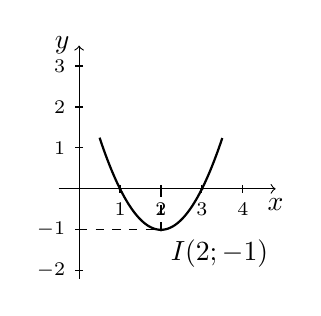
\begin{tikzpicture}[scale=0.52]
    \draw[->] (-0.5,0) -- (4.8,0) node[below] {$x$};
    \draw[->] (0,-2.2) -- (0,3.5) node[left] {$y$};

    \foreach \x in {1,2,3,4}
        \draw (\x,0.1) -- (\x,-0.1) node[below] {\scriptsize $\x$};

    \foreach \y in {-2,-1,1,2,3}
        \draw (0.1,\y) -- (-0.1,\y) node[left] {\scriptsize $\y$};

    \draw[smooth, samples=200, domain=0.5:3.5, thick]
        plot (\x, {\x*\x - 4*\x + 3});

    \fill (1,0) circle (1.3pt);
    \fill (3,0) circle (1.3pt);
    \fill (2,-1) circle (1.3pt);
    \draw[dashed] (2,0) -- (2,-1);
    \draw[dashed] (0,-1) -- (2,-1);
    \node[below right] at (2,-1) {$I(2;-1)$};
\end{tikzpicture}

\end{center}
Xét các khẳng định sau:
\begin{SubQuestions}
  \TFItem{true}{Hàm số có hai nghiệm $x=1$ và $x=3$.}
  \TFItem{true}{Trục đối xứng của đồ thị là đường thẳng $x=2$.}
  \TFItem{false}{Giá trị nhỏ nhất của hàm số bằng $-3$.}
  \TFItem{true}{Bất phương trình $f\left(x\right)\le 0$ có tập nghiệm là $[1;3]$.}
\end{SubQuestions}
\SolutionBlock{Từ đồ thị, parabol mở lên và cắt trục hoành tại $x=1$ và $x=3$, nên hai nghiệm là $1$ và $3$. Trục đối xứng đi qua trung điểm hai nghiệm nên là $x=2$. Đỉnh là $(2;-1)$ nên giá trị nhỏ nhất bằng $-1$, không phải $-3$. Vì parabol mở lên nên $f\left(x\right)\le0$ trên đoạn giữa hai nghiệm, tức là $[1;3]$.}

\NQuestion Trong mặt phẳng tọa độ $Oxy$, cho $A(1;2),\ B(5;-2),\ C(3;4)$. Xét các khẳng định sau:
\begin{SubQuestions}
  \TFItem{true}{$\overrightarrow{AB}=(4;-4)$.}
  \TFItem{true}{Trung điểm của đoạn thẳng $AC$ là $I(2;3)$.}
  \TFItem{true}{Đường thẳng $BC$ có phương trình $3x+y-13=0$.}
  \TFItem{false}{Khoảng cách từ điểm $A$ đến đường thẳng $BC$ bằng $\dfrac{4}{\sqrt{10}}$.}
\end{SubQuestions}
\SolutionBlock{\begin{itemize}[leftmargin=1.5em]
\item Ta có $\overrightarrow{AB}=(5-1;-2-2)=(4;-4)$, nên ý a) đúng.
\item Trung điểm của $AC$ là $I\left(\dfrac{1+3}{2};\dfrac{2+4}{2}\right)=(2;3)$, nên ý b) đúng.
\item Đường thẳng qua $B(5;-2)$ và $C(3;4)$ có hệ số góc $m=\dfrac{4-(-2)}{3-5}=-3$. Suy ra phương trình là $y+2=-3(x-5)\Leftrightarrow 3x+y-13=0$, nên ý c) đúng.
\item Khoảng cách từ $A(1;2)$ đến $BC$ là
\[
d(A,BC)=\dfrac{|3\cdot1+2-13|}{\sqrt{3^2+1^2}}=\dfrac{8}{\sqrt{10}}.
\]
Vì vậy ý d) sai.
\end{itemize}}
